\chapter{Image Segmentation}
\label{ch:image_segmentation}
Initially, the notion of segmentation stands for the process of classifying pixels into groups which corresponds to the same type or class \cite{Margaritondo2011}. The segmentation allows to obtain more meaningful and potentially hidden information from original images, what let to bring indeed numerous insights for various business problems. 

For instance, in medicine analysis segmentation invokes various uses cases such as to measure volume of an organ, to render a 3D view of an organ, surface-based registration and many others. Before moving forward I will explicitly distinguish segmentation types from general point of view.

\begin{figure}[h]
    \centering
    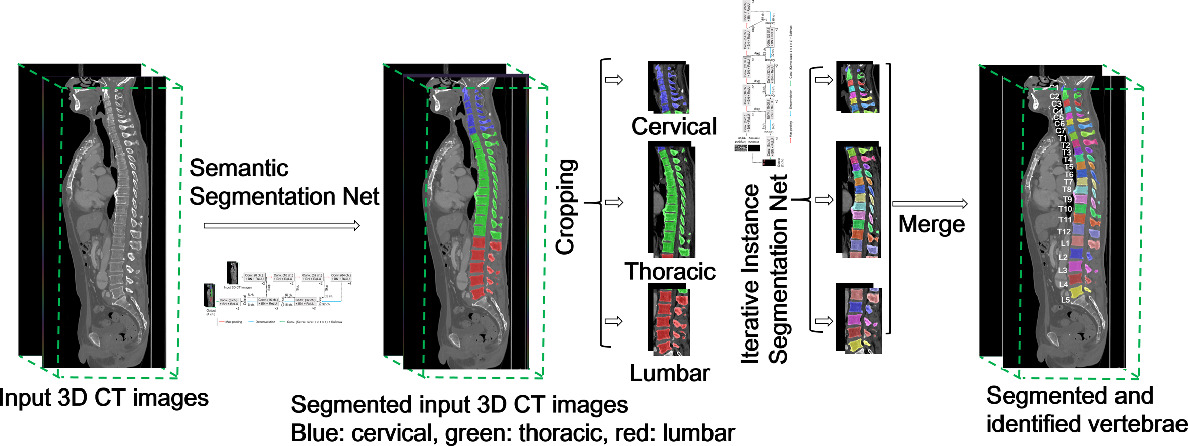
\includegraphics[width=10cm]{images/semantic_instance_segmenattion.png}
    \caption{An example of semantic and instance segmentation.}
    \label{fig:image_segmentation}
\end{figure}

Moving from the left to the right side on the Figure \ref{fig:image_segmentation}, we in deed can transparently notice 2 main types of segmentation. From the very begging there is a original 3D CT image, after applying particular segmentation method, on the second image we see the resulting image where every pixel belongs to a certain class (either blue: cervical, green: thoracic, red: lumbar). Pixels which belongs the same class are represented by the same color. Such type of segmentation is called "semantic segmentation". 

The very last image has assigned a particular class to each pixel of the image as well. However, different objects of the same class have different colors. Such type of segmentation is called "instance segmentation".

\section{Classical Segmentation Methods} 
Now we are good to go with classical segmentation methods section. I will cover basic thresholding method, then modified version of thresholding so called region growing. Afterwards I will speak about edge detection segmentation and clustering based segmentation. On top of that I will demonstrate the performance of each dedicated technique within the following baseline Figure \ref{fig:sample_vertebrae} of vertebrae.

\begin{figure}[h]
    \centering
    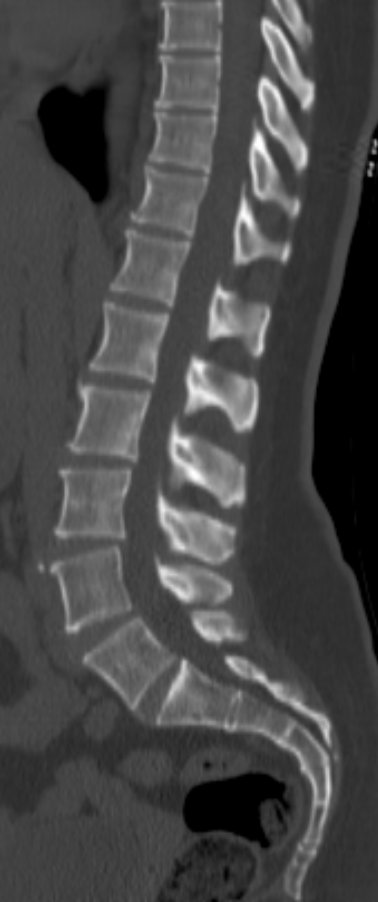
\includegraphics[width=2cm]{images/sample_vertebrae.jpeg}
    \caption{Sample CT scan of vertebrae.}
    \label{fig:sample_vertebrae}
\end{figure}


\subsection{Region Based Segmentation}
Sometimes region based segmentation method is mentioned as thresholding. Actually, it one of the simplest methods for classifying pixels based on solely on their intensity values. In thresholding we have options to choose either upper and lower bound values or to choose just one threshold value which can be for instance the mean of the original image values. 

Mathematically, the algorithm can be defined as:
\[
    f(x, y)= 
\begin{cases}
    0 & \text{, if } f(x, y) > T \\
    255 & \text{, otherwise}
\end{cases}
,\]
where $T$ is threshold value, $x$ and $y$ certain coordinates of pixel.

After applying proposed algorithm with the mean threshold on the baseline Figure \ref{fig:sample_vertebrae}, I had obtained following segmented image depicted on Figure \ref{fig:sample_vertebrae_thresholding}. 

\begin{figure}[h]
    \centering
    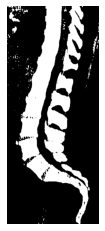
\includegraphics[width=2cm]{images/sample_vertebrae_thresholding.png}
    \caption{Applied thresholding algorithm for sample CT scan of vertebrae.}
    \label{fig:sample_vertebrae_thresholding}
\end{figure}

The problem within simple thresholding is that it does not take into consideration any spatial information of an image, meaning each pixel is evaluated no matter where it is located. Beyond, each time we have to find best way to define either range of values or value for threshold.    


\subsection{Region Growing Segmentation}
Unlike basic thresholding, region growing segmentation indeed takes into consideration spatial information starting with the small set of seed pixels and then growing out from them. 

Let me assume following example. There is set of pixels $4 \cdot 4$ which should be colored (segmented). Some of the cells are already filled with red color, another cells are potential candidates to be segmented. The task is to fill (segment) the "non red" cells with a red color based on predefined thresholding. Mathematically region growing can defined as following equitation: 
\[
    f(x, y) = 
\begin{cases}
    include ,& \text{if } 10 \leq intensity \leq 100 \\
    exclude ,& \text{otherwise}
\end{cases}
\]

All it all, region growing is an iterative method used to extract similar parts of an image. One or several points are chosen as a start. The region then grows until it is finally blocked by the stop criteria. This criteria is generally an inside/outside region comparison such as size or others. 

Exactly the same manner growing region thresholding method can be applied for our \ref{fig:sample_vertebrae_grwoing}.
\begin{figure}[h]
    \centering 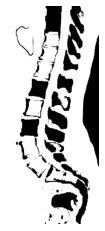
\includegraphics[width=2cm]{images/sample_vertebrae_regiongrowing.png}
    \caption {Applied region growing algorithm for sample CT scan of vertebrae.}
    \label{fig:sample_vertebrae_grwoing}
\end{figure}    

There is a huge potential room for improvements making the method more sophisticated by coming up with different conditions for inclusion/exclusion of pixels.

\subsection{Edge Detection Segmentation}
The detection of edges provides meaningful semantic information that facilitate the understanding of an image. It is often used as auxiliary function or filter to perform segmentation. Edge detection can be used to directly segment edges and regions of images but it is particularly useful when we want to use that as part of another segmentation algorithm.

There are four possible sources of edges in an image: surface normal discontinuity (surface changes direction sharply), depth discontinuity (one surface behind another), surface color discontinuity (single surface changes color), illumination discontinuity (shadows/lighting).

In order to perform edge detection usually it is applied high-pass filters such as Laplacian, Sobel, Prewitt or Canny whereas the corresponding output is so called filter mask which shows the transition values. After filtering it is used thresholding to extract edges.

\subsubsection{Edge Basics}
Edges occur in images when the magnitude of the gradient is high. In order to find the gradient, we must first find the derivatives in both the $x$ and $y$ directions.
\[ \frac{\partial f (x)}{\partial x} = \lim_{\delta{f} \to 0} \dfrac{f(x) - f(x - \delta x)}{\delta x}  = f'(x) \]
\[ \frac{\partial f (x)}{\partial x} = \dfrac{f(x) - f(x - 1)}{1}  = f'(x) \]
\[ \frac{\partial f (x)}{\partial x} = f(x) - f(x - 1) = f'(x) \]

It is also possible to take the derivative in three different ways and represent them as filter (convoluting the filter with the image gives the derivative) as:
\begin{align*}
Backward: f'(x) = f(x) - f(x - 1) \to [0, 1, -1] \\
Forward:  f'(x) = f(x + 1) - f(x) \to [-1, 1, 0] \\
Central:  f'(x) = \dfrac{(x + 1) - f(x - 1)}{2} \to [1, 0, -1]
\end{align*}

The gradient ($\nabla f$), gradient magnitude ($|\nabla f(x, y)|$) and gradient angle ($\Theta$) can be accordingly calculated as: 
\begin{align*}
\nabla f(x, y) = [ \frac{\partial{f (x, y)}}{\partial{x}}, \frac{\partial{f (x, y)}}{\partial{y}} ]  = [f_x, f_y] \\
|\nabla f(x, y)| = \sqrt{f^2_x + f^2_y} \\
\Theta = \tan^{-1} \frac{f_y}{f_x}
\end{align*}

\subsubsection{Convolution}
Convolution itself is a mathematical operation on two functions ($f$ and $g$) that produces a third function $f \cdot g$ that expresses how the shape of one is modified by the other. In other words, convolution can be described as the filter is sliding, or convolving, around the input image, it is multiplying the values in the filter with the original pixel values of the image (aka computing element wise multiplications). These multiplications are all summed up. In mathematical terms the output size of convolution operation is: \[ \text{size of output volume} = \frac{W-F+2 \cdot P}{S+1} \] where $W$ - is the input volume size, $F$ - is the receptive field size, $S$ - the stride with which they are applied and $P$ - is the padding.

Let me show how actually convolution operation works. Assume we have 1 channel image size of $5 \cdot 5$ as shown on the Figure \ref{fig:sample_1_channel_image} below.
\begin{figure}[h]
    \centering 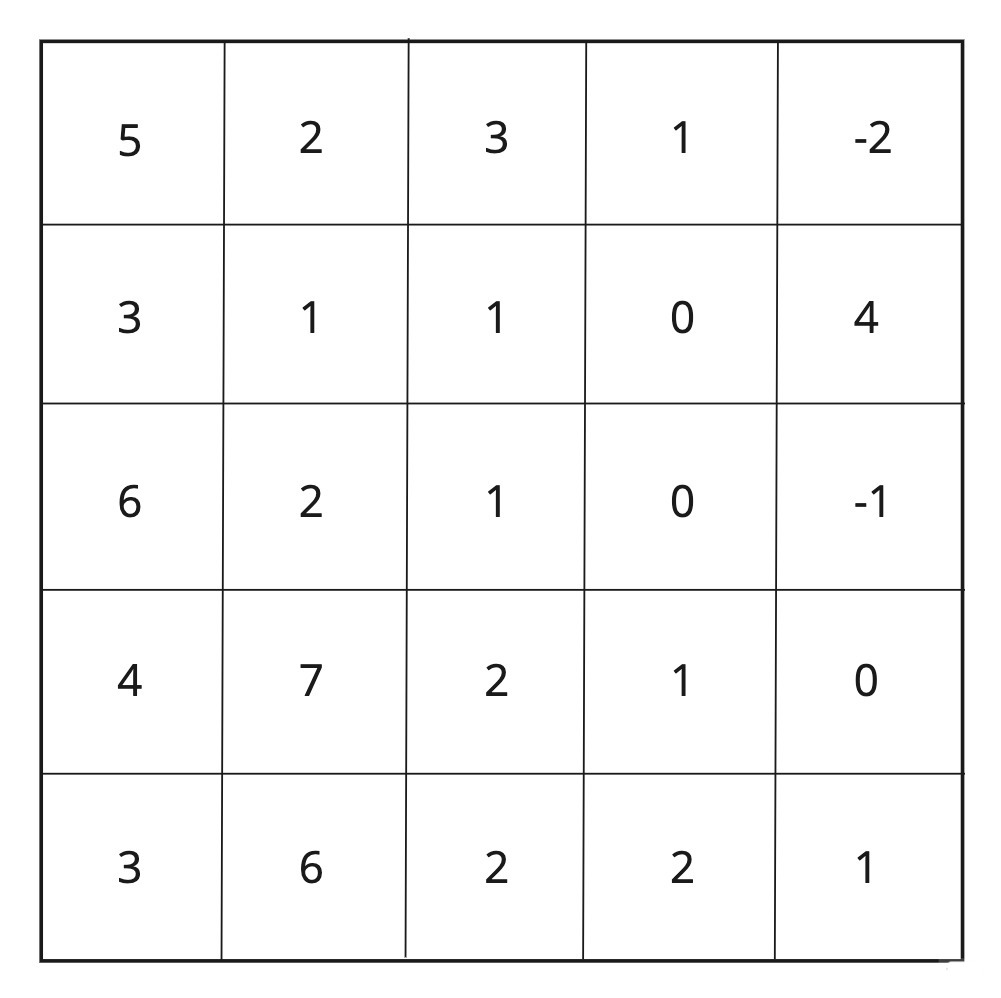
\includegraphics[width=5cm]{images/1_channel.jpg}
    \caption {Sample 1 channel image.}
    \label {fig:sample_1_channel_image}
\end{figure}

And the filter (kernel) which I had defined as: 
\[ \begin{pmatrix} 1 & 0 & -1 \\ 0 & 1 & 0 \\ -1 & 0 & 1 \end{pmatrix} \]

We need to calculate the convolution with the custom filter (kernel) size of $3 \cdot 3$, padding $1 \cdot 1$ and stride $1$.
\begin{figure}[h]
    \centering 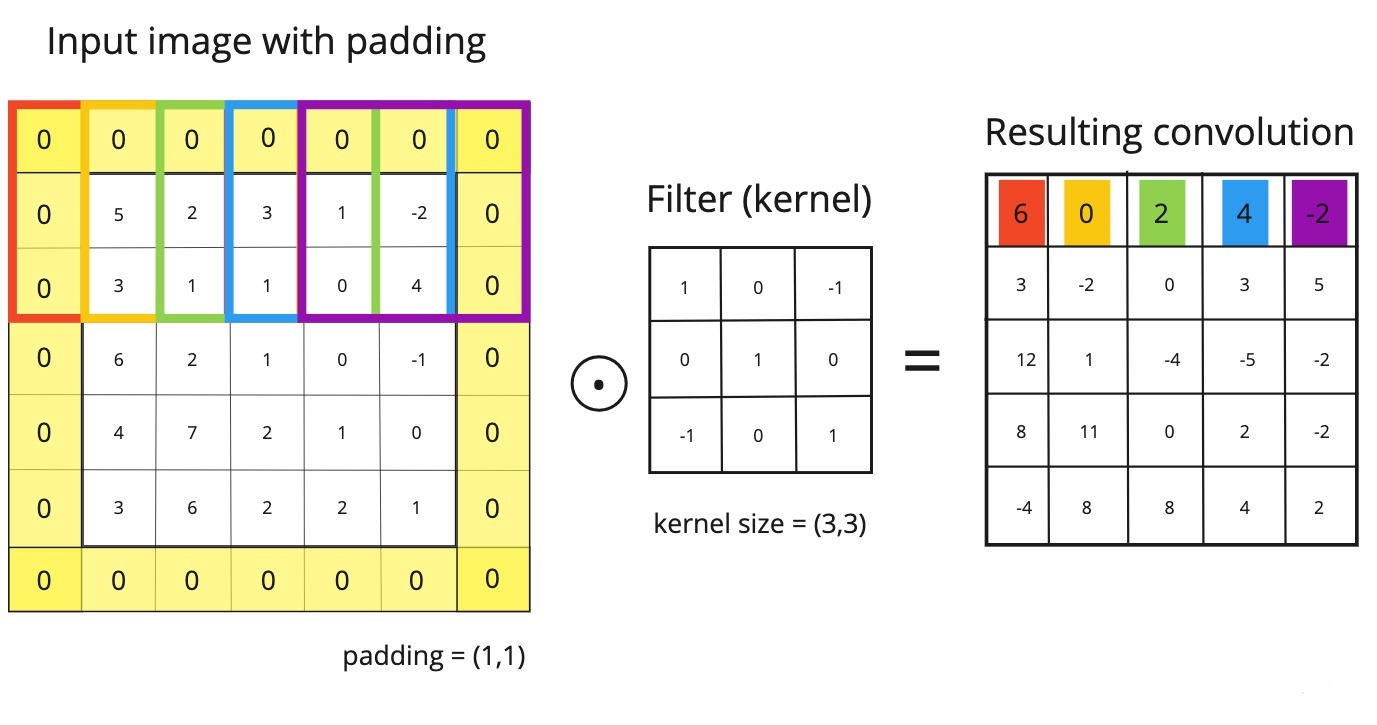
\includegraphics[width=10cm]{images/convolution_operation.jpeg}
    \caption {Example of convolution operation.}
    \label{fig:convolution}
\end{figure}

The illustration of obtaining of the red colored cell on the resulting convolution depicted on Figure \ref{fig:convolution} can be calculated as:    
\[ \begin{pmatrix} 0 & 0 & 0 \\ 0 & 5 & 2 \\ 0 & 3 & 1 \end{pmatrix} \odot \begin{pmatrix} 1 & 0 & -1 \\ 0 & 1 & 0 \\ -1 & 0 & 1 \end{pmatrix} = \]
\[ = 0 \cdot 1 + 0 \cdot 0 + 0 \cdot (-1) + 0 \cdot 0 + 5 \cdot 1 + 2 \cdot 0 + 0 \cdot (-1) + 3 \cdot 0 + 1 \cdot 1 = \] 
\[ = 0 + 0 + 0 + 0 + 5 + 0 + 0 + 0 + 1= 6 \]
I have just calculated convolution for particular pixel of the image. 

\subsubsection{Sobel Filter}
Now I can emphasize that each filter utilizes various functionalities described above.
For instance, Sobel filter performs on our baseline image as shown on Figure \ref{fig:sobel}.

\begin{figure}[h] 
\centering
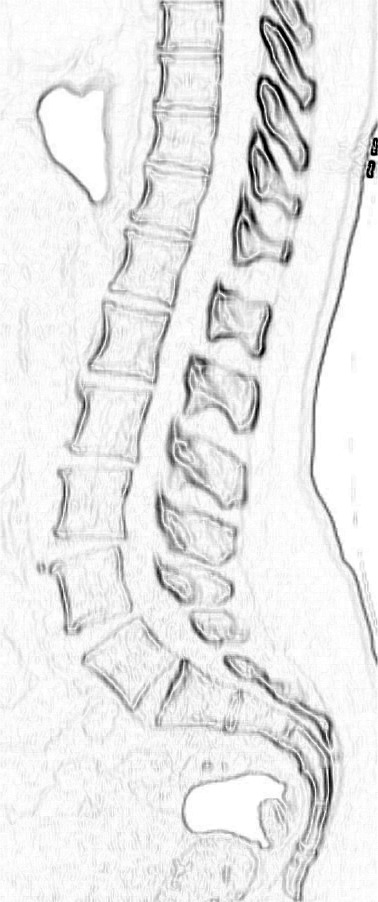
\includegraphics[width=2cm]{images/sample_vertebrae_sobel.jpeg}
    \caption {Applied Sobel filter for sample CT scan of vertebrae.}
    \label{fig:sobel}
\end{figure}

In general, each edge detector can be either separate convolution operation within special filter and threshold or combination such as: suppressing noise, computing gradient magnitude and direction, applying non-maximum suppression, applying hysteresis thresholding and finally utilizing connectivity analysis to detect edges (Canny Edge Detector). 

By the reason of edge detection is based on derivatives it can easily degrade with variations and noise. But issues which should be considered are size of the neighborhood as well as what exactly represents a transition on the image. 

\subsection{Segmentation Based on Clustering}
The obvious question I can ask myself whether I can use clustering techniques to divide images into segments. And the answer is - yes, I can! All it all, the aim is to group objects (instances) into so-called clusters, such that objects in the same cluster are (or, at least, should be) more similar to each other than to the objects belonging to other clusters. 

Within clustering there are multiple algorithms to be issued. Few of them are 
Dynamic Time Warping, Hierarchical Agglomerative Clustering and k-Means. Beyond it should be intuition behind what is similarity in terms of clustering, but I will not cover this part, instead focus on most popular and in the public eye algorithm so called k-Means.  

k-Means algorithm is a common and simple clustering method whereas usually the data set is represented as the a scatter plot in some feature space.

The Figure \ref{fig:triangle} and Figure \ref{fig:clustering} helps to understand how indeed images data can be represented in some feature space. On the Figure  \ref{fig:clustering} depicted the representation of colored triangle in 3D space, where each dimension represents each color.

\begin{figure}[h]
    \centering
    \begin{minipage}[b]{0.4\textwidth}
    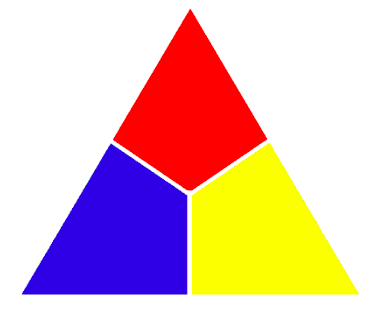
\includegraphics[width=\textwidth]{images/k_mean_triangle.png}
    \caption{Colorful triangle.}
    \label{fig:triangle}
    \end{minipage}
    \hfill
    \begin{minipage}[b]{0.4\textwidth}
    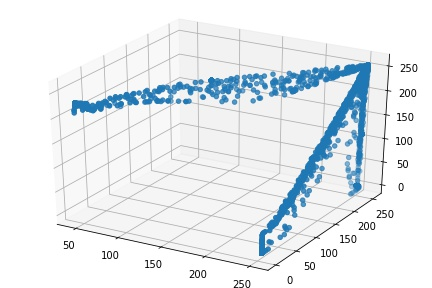
\includegraphics[width=\textwidth]{images/k_mean_triangle_clustered.jpg}
    \caption{Feature space representation.}
    \label{fig:clustering}
    \end{minipage}
\end{figure}

Considering mathematically, given $D \subseteq D_1 \times D_2 \times ... \times D_m$, a distance measure $d$ (or similarity measure $s$) and the number of clusters $k$, where $k \ll n$. The goal is to find cluster centers $c_1, c_2, ..., c_k$ and a mapping $p: D \rightarrow {1, 2, .., k} $ such that \[ \sum_{i=1}^{n} d(x_i, c_p_{x_i}) - \text{is minimal}\]

The algorithm itself can be assumed as:
\begin{itemize}
    \item Initialize $c_1, c_2, ..., c_k$ such that for all $i = {1, 2, .., k}$
    \subitem $c_i \in D$ (random initialization), or
    \subitem or $c_i = \frac{\sum_{x, p(x) = x^X}}{\sum_{x, p(x) = x^1}}$
    \item compute $p$ such that
    \subitem $\sum_{i=1}^n d(x_i, c_p_{(x_i)})$ is minimal
    \item update $c_i$ for all $i = {1,2, ..., k}$ where changed then goto step 2
    \item return $p$ and $c_1, c_2, ..., c_k$
\end{itemize}
    

To demonstrate the method performance I will proceed with the same baseline CT spine scan which had used for region growing thresholding. As for regressors number (number of clusters) I had chosen $k=3$.  

\begin{figure}[h]
    \centering 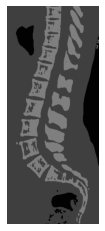
\includegraphics[width=2.5cm]{images/sample_vertebrae_kmeans.png}
    \caption {Applied k-Means algorithm for sample CT scan of vertebrae.}
\end{figure}

Eventually, as results show, clustering is a really "good to go" way for image segmentation, but there are various disadvantages such as tackling with number of clusters, being dependent on initial values, clustering outliers and scaling with number of dimensions.

\section{Modern Segmentation Methods}
Previously, I have covered classical approaches including machine learning ones for image segmentation. Now I would like to narrate about recent techniques which live under umbrella of deep learning family.        

\subsection{Deep Learning Basics}
For simplicity I will represent neuron's mathematical model graphically on Figure \ref{fig:neuron}. It should be taken into consideration, the red characters denote tune parameters of the neuron.     

In the mathematical model of the neuron, the body of the neuron, where the input signals accumulates, is denoted by a summarizing neuron. In addition, the biological neuron also has axons and dendrites, which get the inputs and send the outputs. 

\begin{figure}[h]
    \centering 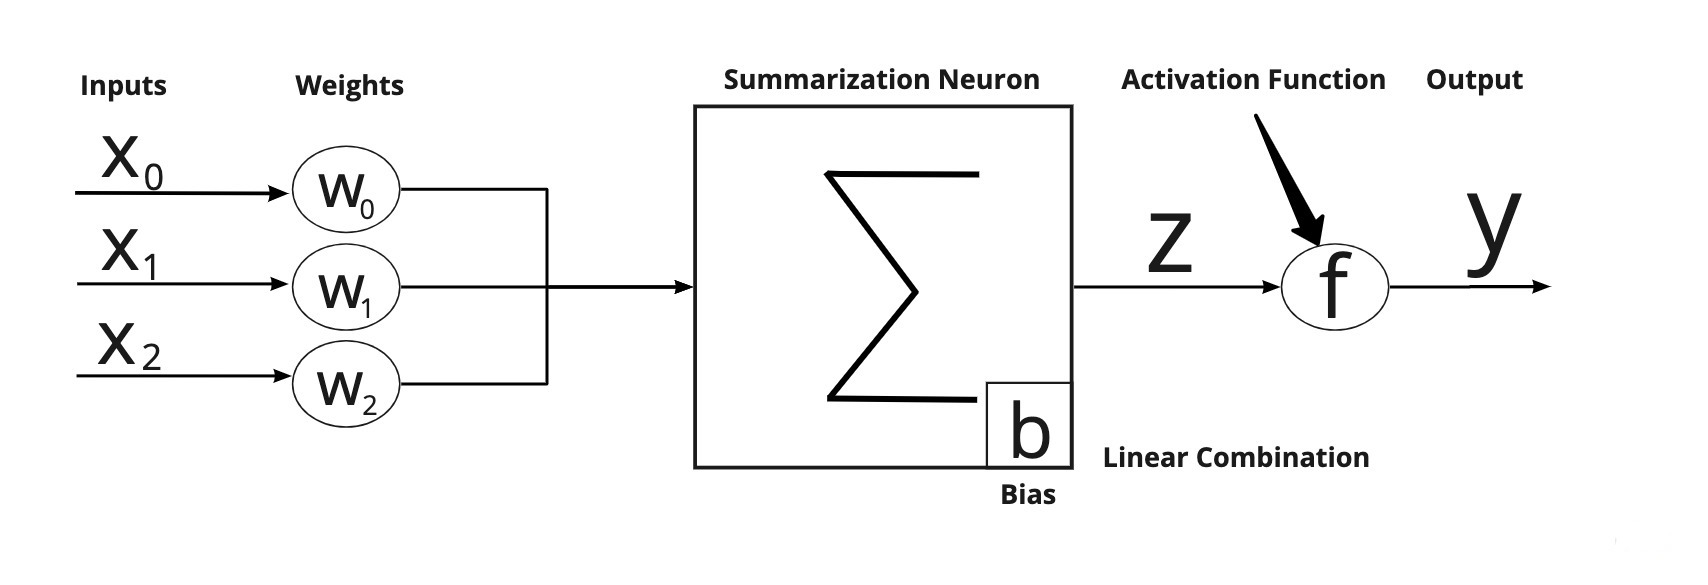
\includegraphics[width=10cm]{images/neuron_math_model.jpeg}
    \caption {Mathematical model of neuron.}
    \label{fig:neuron}
\end{figure} 

Accordingly, in our mathematical model of the neuron, we will add inputs and outputs to the summarizing neuron. It is also worth to keep in mind the biological neuron applies some actions with the signals that come into it, namely, it accumulates charge until it reaches some threshold and only after that forwards it further. This is what we will do in the mathematical model of the neuron using the activation functions.

Mathematical definition of neuron's model:
\begin{align*}
y = f(z) = f(w_0 \cdot x_0+w_1 \cdot x_1+w_2 \cdot x_2+b) = f(\sum\limits_{i=0}^{N-1} w_i \cdot x_i+b) = f(\langle w, x \rangle + b)
\end{align*}
Where: $x_0, x_1, x_2$: inputs, $w_0, w_1, w_2$: weights,  $b$: some bias for increasing non-linearity, $f(z)$: some activation function. 

Inputs can be either single number or vector of numbers. As for weights, we mainly should remember they are tuned parameters. Moreover it should be considered 2 potential situations to manage with. The first one is initialization of the weights. Here we have multiple options whereas we literally can define them either randomly or apply special initialisation techniques such as 'He' initialization or 'Xavier' initialization and others. The second situation we should be aware of is to somehow change the weights during model fitting, meaning weights should be changed in iterative manner from epoch to epoch. To do this we will apply backpropagation algorithm. Concerning the bias, which is like a weights, meaning tuned parameter, we can consider it allows to shift the activation function by adding a constant to the input of neuron. Hence, the last but not least component is activation function. In simplified terms, activation function is used to determine the output of neuron in a manner: 'yes' or 'no'. It maps the resulting values in range between 0 to 1 or -1 to 1.            

\subsubsection{Activation Function}
There is a significant number of various activation functions. Let me assume the very basic one named 'step function' and figure out from general point of view how it works in both mathematical and geometrical sense.   
The 'step function' is defined as:
\begin{align*}
f(x) = \begin{cases} 0, & \mbox{if } x\mbox{ $\leq$ 0} \\ 1, & \mbox{if } x\mbox{ $>$ 0} \end{cases}
\end{align*}

The function has 2 strongly distinguished values: $0$ and $1$. The place where the function changes it's value from $0$ to $1$ is named as dividing surface. Hence, the dividing surface place is where the argument of activation function is equal $0$.

\begin{figure}[h]
    \centering 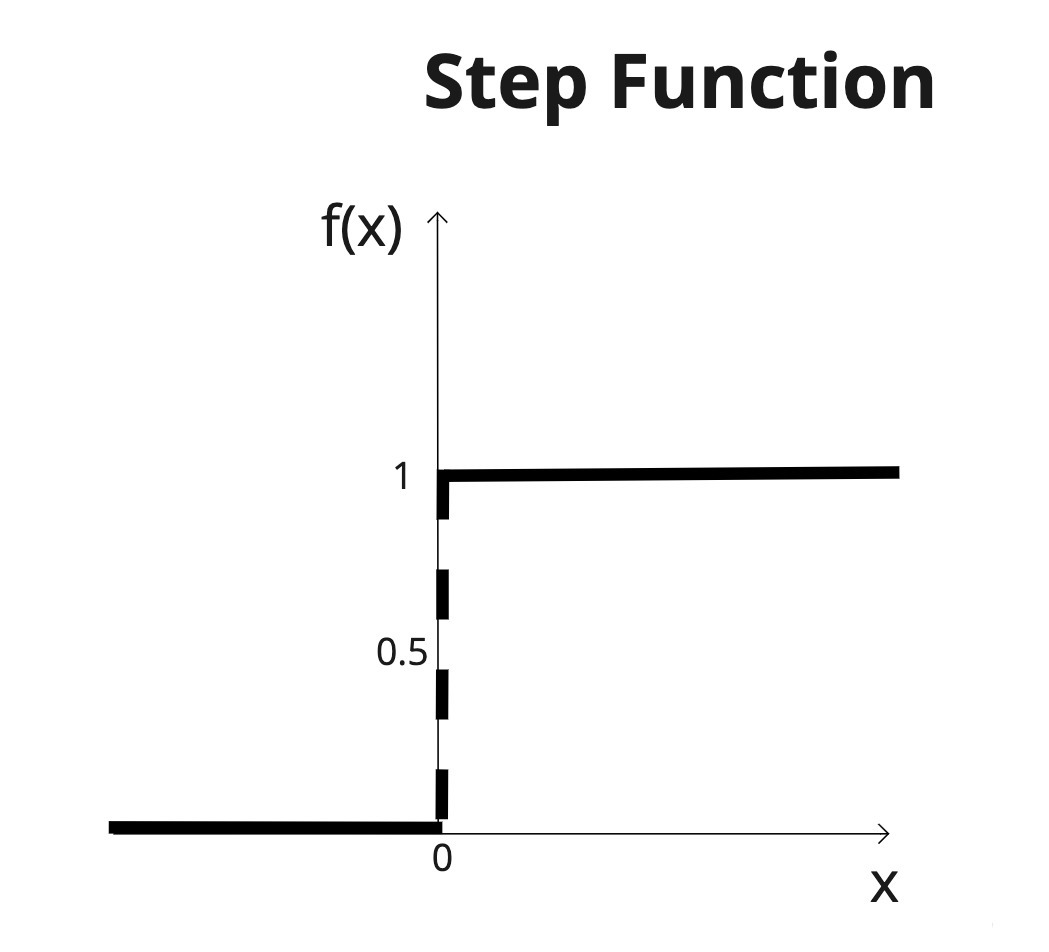
\includegraphics[width=7cm]{images/step_function.jpeg}
    \caption {Geometrical representation of step function.}
\end{figure}

The geometrical representation of step function can be derived as following. Assume there is the neuron formula:
\begin{align*}
y = f(\langle w, x \rangle + b)
\end{align*}

The neuron does some linear operation, which is denoted by 2 parameters: $w$ (vector of weights) and $b$ (bias).

Accordingly, the dividing surface is defined by following equitation which denotes equitation of straight line:

\begin{align*}
\langle w, x \rangle + b = 0
\end{align*}

On one hand the value of step function is equal $1$ and from the opposite $0$. The activation function is equal $1$ that side of dividing surface where the vector $w$ points out. From geometrical point of view it is represented on Figure \ref{fig:dividing_surface}.  

\begin{figure}[h]
    \centering 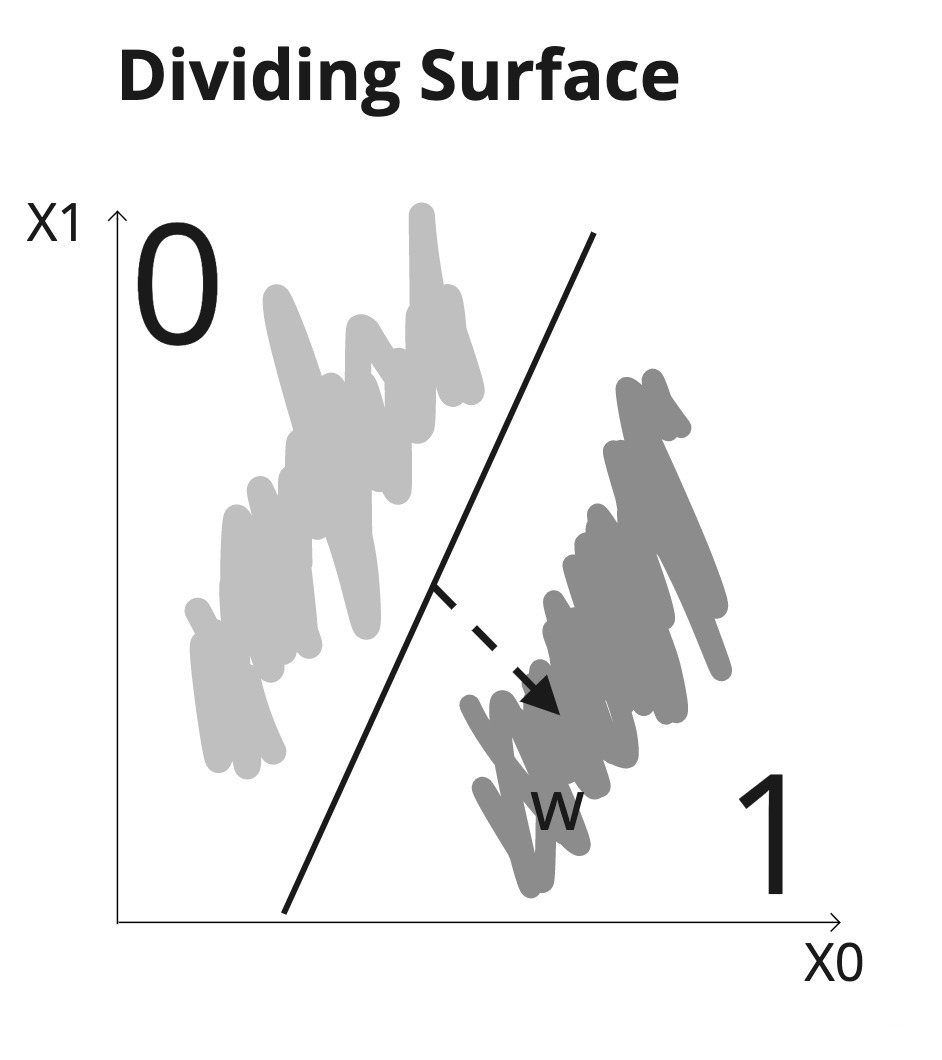
\includegraphics[width=6cm]{images/dividing_surface.jpeg}
    \caption {Sample geometrical representation of dividing surface for single neuron.}
    \label{fig:dividing_surface}
\end{figure}

As it was mentioned earlier, there are many more functions. For instance sigmoid activation function showed on Figure \ref{fig:sigmoid} which unlike step function does not have discontinuity point at zero. 

\begin{figure}[h]
    \centering 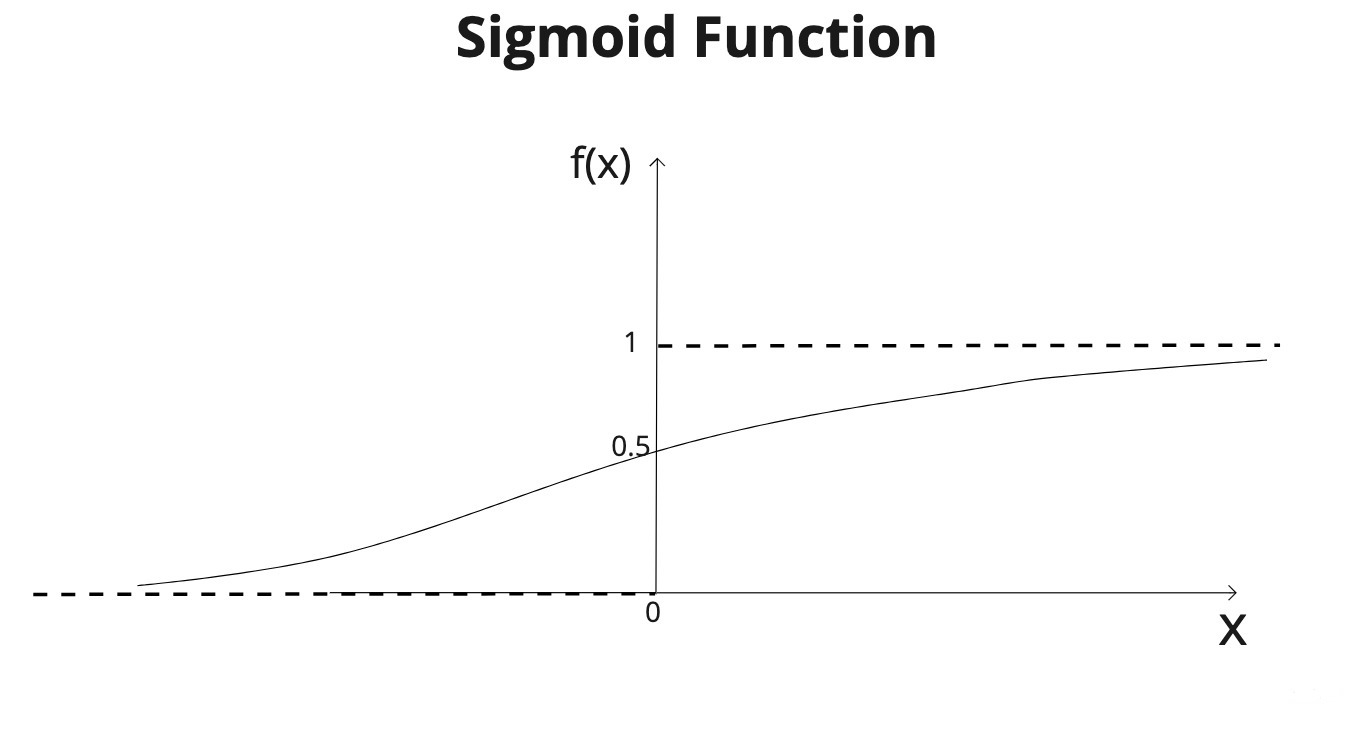
\includegraphics[width=10cm]{images/sigmoid_function.jpeg}
    \caption {Sigmoid activation function.}
    \label{fig:sigmoid}
\end{figure}

The sigmoid activation function formed as:
\begin{align*}
\sigma(x) = \dfrac{1}{1+e^x}
\end{align*}

\[ \sigma(x) = \begin{cases} 1, & \mbox{if } x\mbox{$\xrightarrow{} + \infty$} \\ 0, & \mbox{if } x\mbox{$\xrightarrow{} - \infty$} \end{cases} \]

One more activation function is rectified linear activation function. For short it is a piece-wise linear function which outputs input directly if it is positive otherwise outputs zero. It has become the common-wise activation function for many types of neural networks.

\subsubsection{From Neuron to Neural Network}
So far I have covered the properties and functional of just a single neuron, which as a result outcomes a linear divide surface unlike multiple neurons as shown on Figure \ref{fig:dividing_surface}, meaning when we concatenate the multiple neurons in some architecture we may achieve some nonlinear divide surfaces.
\begin{figure}[h]
    \centering 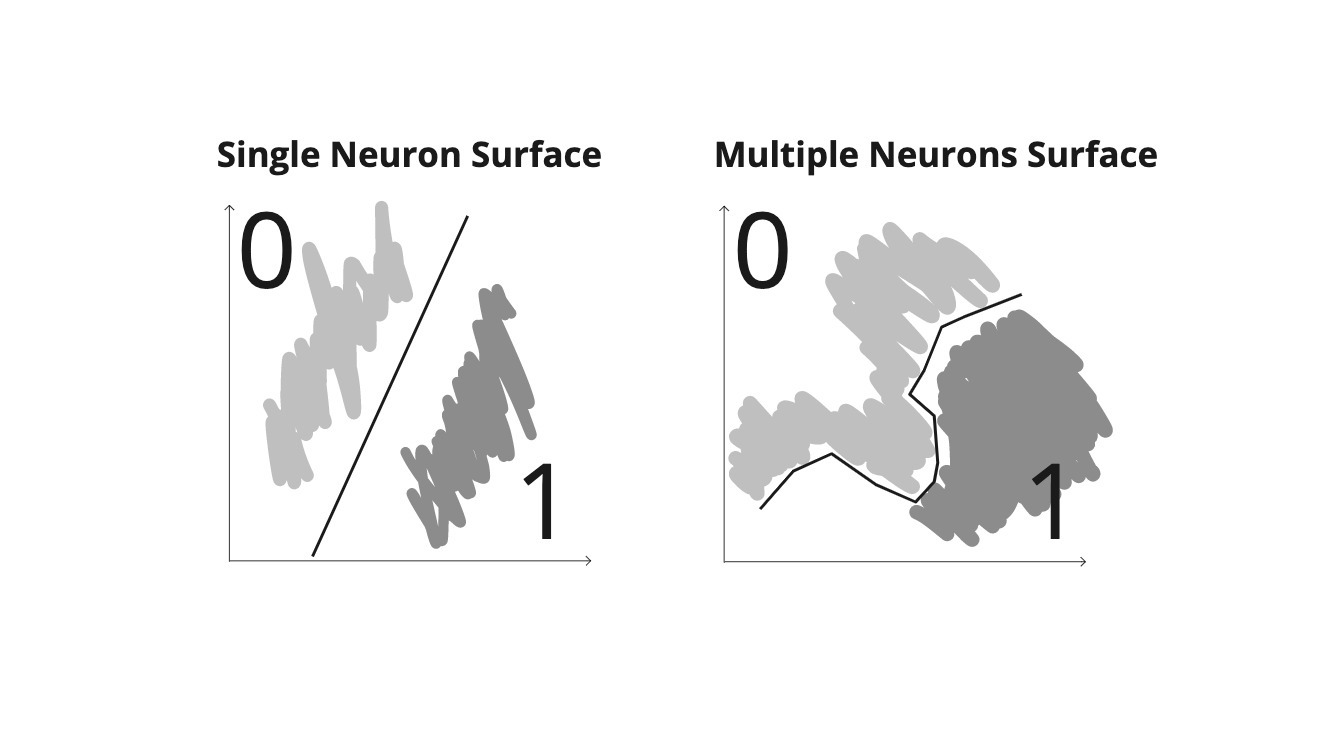
\includegraphics[width=10cm]{images/neuron_to_neural_net.jpeg}
    \caption {Sample geometrical representation of dividing surface for single neuron versus multiple neurons.}
    \label{fig:dividing_surface}
\end{figure}

Now the question is how do we get the nonlinear dividing surface. Simply put, define 3 neurons with linear activation function as shown on Figure \ref{fig:1_layer_net}. 

\begin{figure}[h]
    \centering 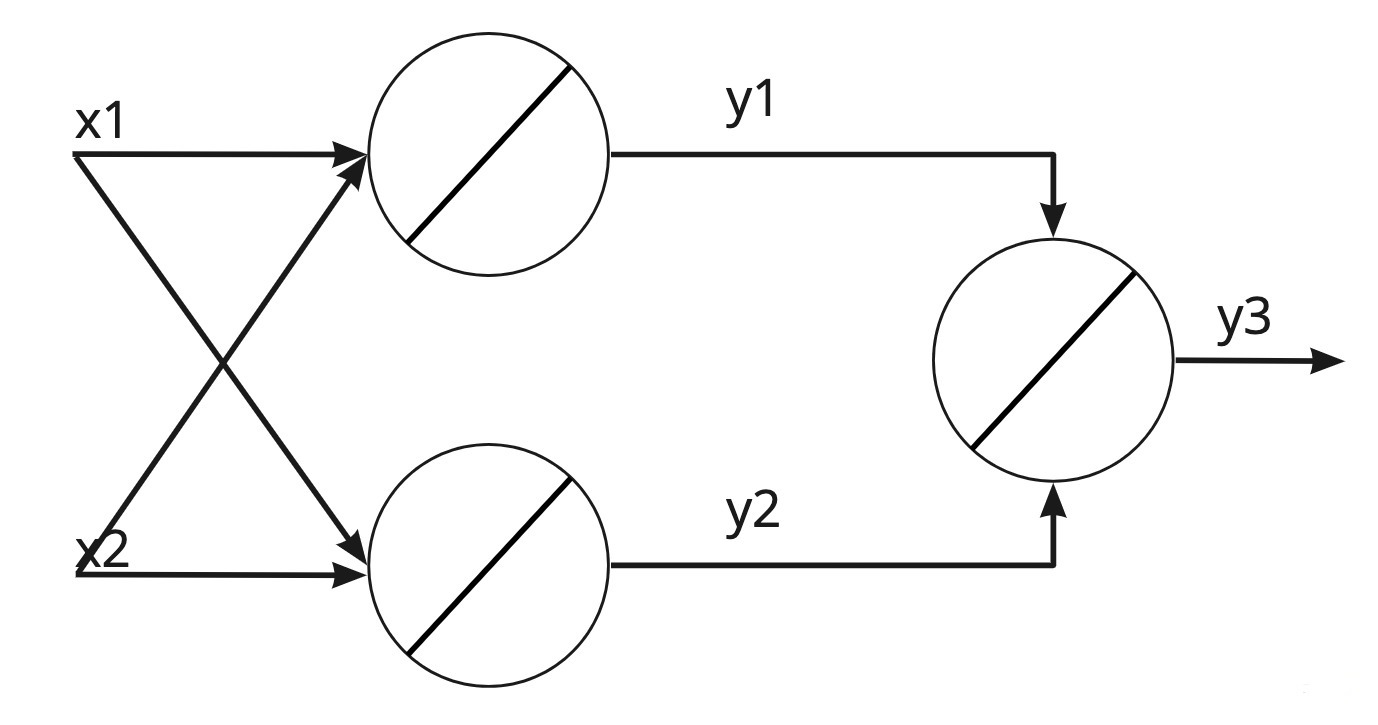
\includegraphics[width=6cm]{images/3_neurons_net.jpeg}
    \caption {Sample 1 layer neural net with linear activation functions.}
    \label{fig:1_layer_net}
\end{figure}

The results of performing the net can be considered as:
\[ y_3 = f(w_2^3 \cdot y_2+w_1^3 \cdot y_1+b^3) = \]
By the reason $f$ is simple linear function, equation can be derived as:
\[ = w_2^3 \cdot y_2+w_1^3 \cdot y_1+b^3 = \] 
\[ = w_2^3 \cdot f(w_2^1\cdot x_1+w_2^2 \cdot x_2+b^2) + w_1^3 \cdot f(w_1^1 \cdot x_1+w_1^2 \cdot x_2+b^1) + b^3 = \]   
\[ = w_2^3 \cdot w_2^1 \cdot x_1+w_2^3 \cdot w_2^2 \cdot x_2+b^2 + w_1^3 \cdot w_1^1 \cdot x_1+w_1^3 \cdot w_1^2 \cdot x_2+b^1+b^3 = \]
\[ = x_1[w_2^3 \cdot w_1^2 + w_1^3 \cdot w_1^1] + x_2[w_2^3 \cdot w_2^2 + w_1^3 \cdot w_2^1] + [w_2^3 \cdot b^2+w_1^3 \cdot b^1+b^3] = \]
\[ =  x_1\cdot \tilde{w_1} + x_2\cdot \tilde{w_2} + \tilde{b} \]
Meaning the obtained result is just linear combination of inputs into the neural net. 
\subsubsection{Loss function}
Characteristically neural networks we keen to minimize the error. There are many functions that could be potentially used to estimate error of set of weights in a neural network. Below we consider few popular loss functions.

Mean Squared Error is the average of the squared error that is used as the loss function for least squares regression. To streamline, MSE is the sum,over all the data points of the square of the difference between the predicted and actual target variables divided by the number of data points.
\begin{align*}
\text{MSE} = \frac{{1}}{n} \sum_{i=1}^{n} (y_i - \widehat{y_i})^2
\end{align*}
where $y$ is the desired Neural Network output, and $\widehat{y_i}$ is the neural network output.

Frequently, jointly loss functions it is utilized different regularization terms. The purpose of regularization terms is establish additional rules for penalizing the loss function for errors. Meaning the regularization will manage whether the weights are important (good) or not. One of such regularization techniques is L2 regularization or so called weight decay. The definition is as:
\[ \lambda \cdot \sum_{i=1}^{n} \alpha_i^2 \]

In terms of mean squared error loss function, the addition of regularization considered as:
\[ \sum_{i=1}^n(\hat{y}-y_i)^2 + \lambda \cdot \sum_{i=1}^{n} \alpha_i^2\]

One more commonly used function is so called cross-entropy loss, or log loss. It measures the performance of a classification model whose output is a probability value between 0 and 1. Cross-entropy loss increases as the predicted probability diverges from the actual label. For discrete probability distributions $p$ and $q$ with the same support $X$ this means over a given set is defined as follows:
\[H(p,q) = - \sum_{x \in X} p(x) \log q(x) \]


\subsubsection{Gradient Descent}
Optimization of neural net is the key component in terms of fitting a model. The optimization of the net should be considered as the on-the-spot training. There are variety of optimization algorithms but the pillar algorithm in the list is gradient descent.

Suppose a function which is defined by some levels lines as shown on Figure \ref{fig:gradient}. The function has 2 minimums, which are denoted by the red dots.  It worth to understand by distancing from the minimums the function value increases. 
So far, we have a neural net with some parameters (weights and biases) which performs some value of loss function. As we remember the task is to decrease the value of loss function. Hence, the question is how to do that ? 

\begin{figure}[h]
    \centering 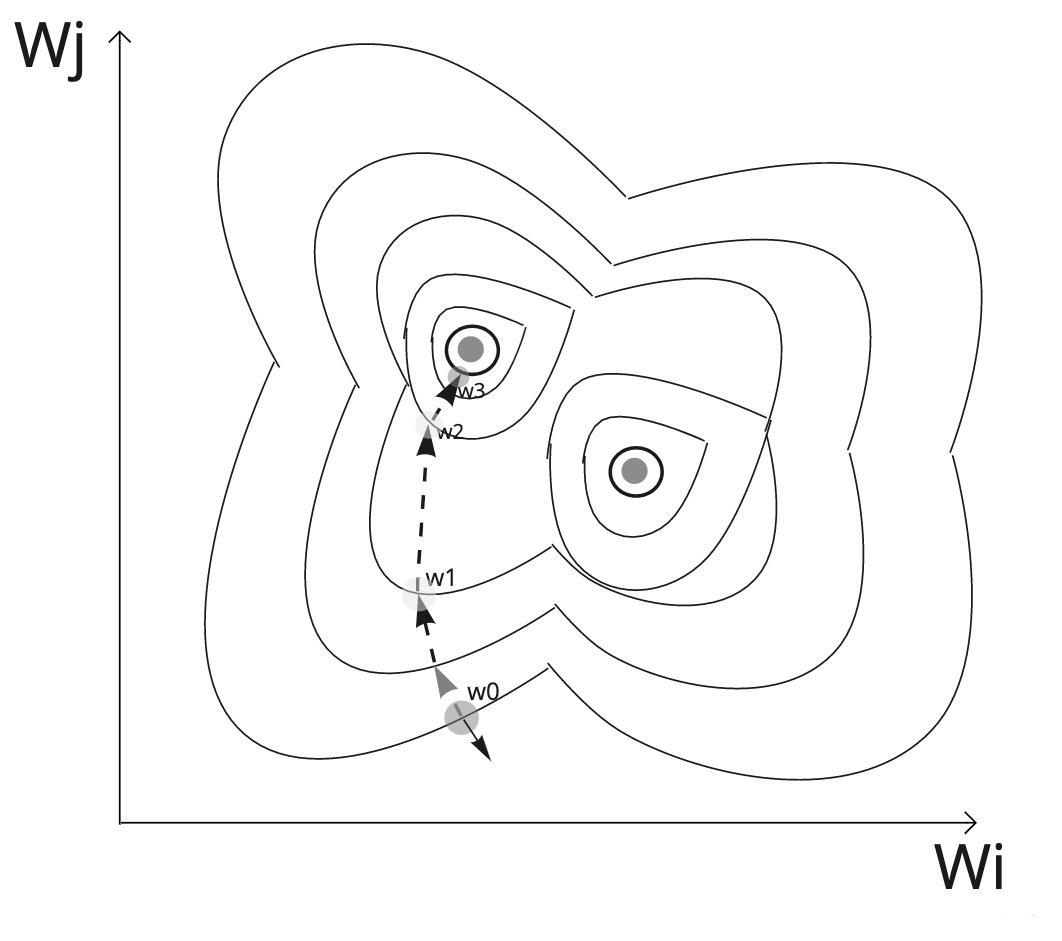
\includegraphics[width=9cm]{images/gradient_descent.jpeg}
    \caption {Sample gradient descent visualization.}
    \label{fig:gradient}
\end{figure}

So, the very first provision in the vector of function surface will be defined by $w_0$, where $w_0$ denotes vector of all weights and biases of the net and can be represented as: 

\[ w_0 = [w_1^1, w_1^2,...,w_1^n, w_2^1,...,w_2^n,...,w_n^n, b1^1, b1^2,...,b1^n, b2^1,...,b2^n,...,b_n^n] \]

Accordingly, we need take derivative (meaning gradient, which is vector consisting of derivatives per each coordinate of the function) of the loss function of our vector. It can be represented as:
\[ \delta{f} = \left[ \frac{\partial{f}}{\partial{w_0}}, \frac{\partial{f}}{\partial{w_1}}, ... ,\frac{\partial{f}}{\partial{w_n}} \right] \]
As the result, we have calculated the gradient of loss function at the point ($w_0$) where we currently located. The gradient of loss function points out at the direction of greater loss function growth. But, oppositely, we on demand of lower loss function growth, meaning we need to make an opposite step of calculated gradient descent. It can be considered as:
\begin{align*}
w_1 = w_0 - \alpha \cdot \delta{f(w_0)}
\end{align*}
where $w_0$: the initial vector of weights and biases of neural net, $\alpha$: parameter for regulating the 'speed' of training the neural net. In other words it affects the size of gradient step and $\delta{f(w_0)}$: calculated gradient of loss function at the $w_0$ point. 

The gradient descent of loss function will be calculated until it will not converge some preciseness within predefined fallacy.

\subsection{Convolutional neural networks (CNN)}
So far I have wrapped up the very basics behind neural networks what can be considered as feed forward neural nets. The cons of such typed neural networks are that they can perfectly find the latent consistencies however they struggle structured data such as images.

To distinguish feed forward and convolution nets, suppose, there is an RGB image sized $224 \cdot 224$ where a dog is located in the middle of image. The goal is to classify whether the dog is on the image. The usual (for instance sigmoid feed forward) neural network will come up with the mask of the dog based on the image. But once new image will be revealed and the dog will not be located in the middle of it, the net will not be able to find and classify the dog. Whilst convolutional neural networks could be generalized independently of the location of the dog, because the convolution itself is invariant operation.         

There are few more essential properties within CNNs such as pooling, dropout and others, but I'm aim to focus on architectures themselves and their performance. 

\subsection{Unet}
The U-net is convolutional network architecture for fast and precise segmentation of images. It was proposed by Olaf Ronneberger, Philipp Fischer, and Thomas Brox at 2015 \cite{Ronneberger2015}. 

\begin{figure}[h]
    \centering 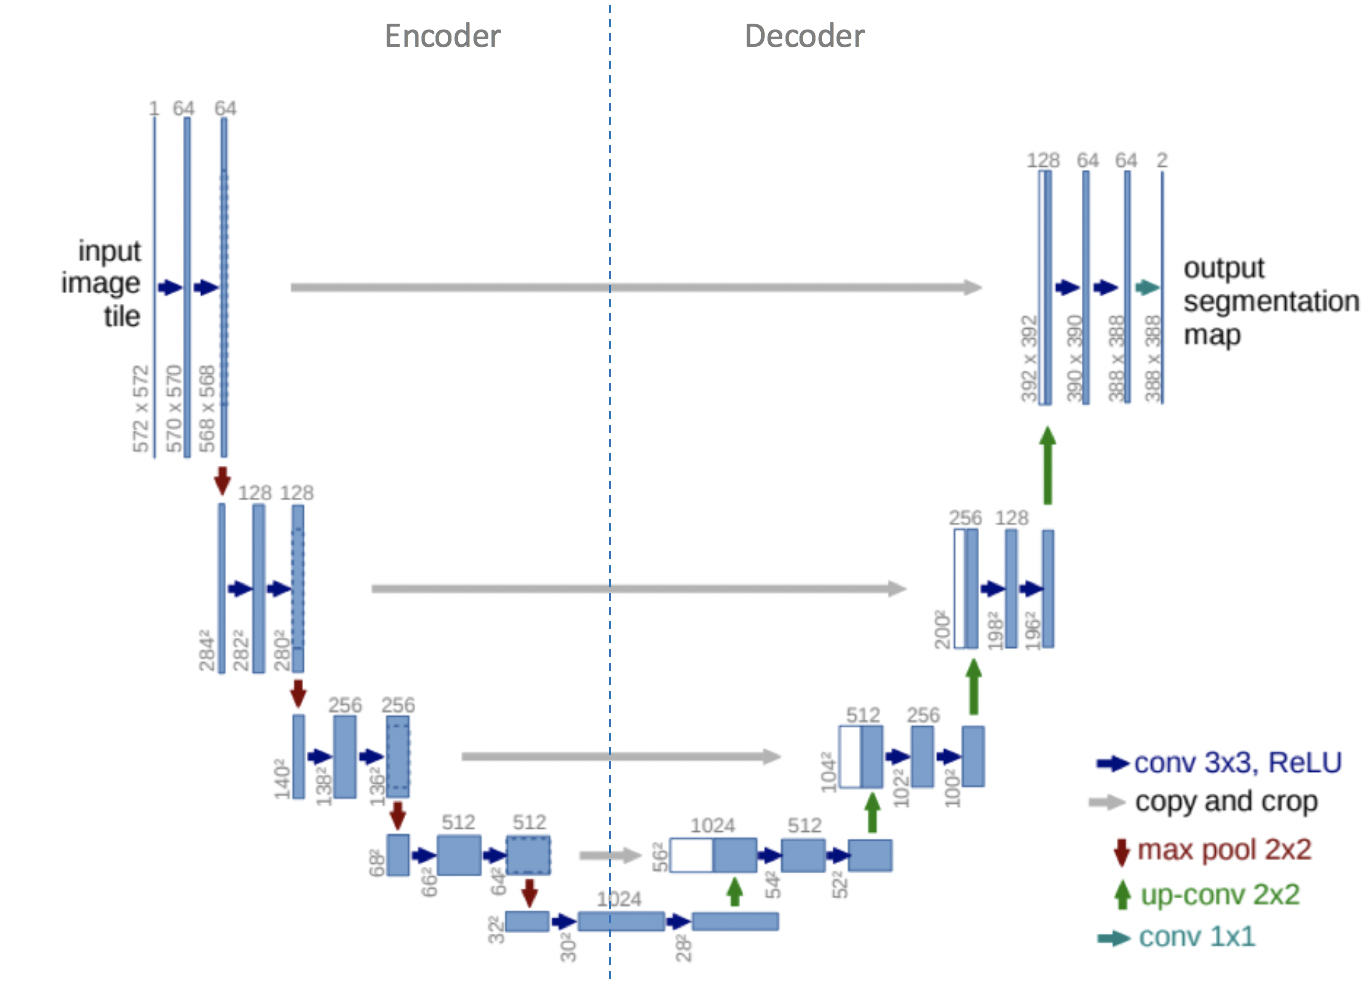
\includegraphics[width=10cm]{images/unet.png}
    \caption {Unet architecture.}
    \label{fig:unet}
\end{figure}

Using original terminology of the authors \cite{Ronneberger2015} the net consist of a contracting path (left side) and an expansive path (right side) as shown on Figure \ref{fig:unet}. The contracting path follows the typical architecture of a convolutional network. In simplified terms it can be considered as downsampling or encoder which formed as
a five repeats of double $3 \cdot 3$ convolutions (unpadded convolutions) with rectified linear unit and $2 \cdot 2$ max pooling operation with stride 2. Thus expansive path which can be considered as upsampling or decoder consists of 4 repeats of double $2 \cdot 2$ convolutions (up-convolution) which halve number of feature channels. In total the network has 23 convolutional layers. 

Lastly mentioning, U-net proved itself multiple times and still is one of the main backbone architectures for medical images analysis. As Ahmed \cite{Ahmed2020} observed in his "Comparison results of segmentation models using top view person data set." work, U-net still remains one of the best ones.  

\begin{table}[htbp]
\centering
\begin{tabular}{|l|c|c|c|c|c} \hline\hline
Method & Precision & Recall & F1-score & Pixel Accuracy\\ \hline
Otsu & 50\% & 80\% & 70\% & 78\%  \\
Watershred & 52\% & 82\% & 74\% & 80\% \\
Gaussian mixture-based model & 60\% & 82\% & 76\% & 82\%  \\
Background subtraction-based model & 65\% & 84\% & 74\% & 84\% \\
RE-weighted HOG & 68\% & 82\% & 75\% & 82\%  \\
FCN & 62\% & 92\% & 76\% & 91\%  \\
U-net & 74\% & 92\% & 81\% & 92\% \\
DeepLabV3 & 80\% & 96\% & 83\% & 93\% \\ 
\hline\hline
\end{tabular}
\end{table} 


\subsection{DoubleU-Net}
The doubleU-net is enhancement wrapper over U-net, which make the architecture less flexible but more scope-wise related. It consists of 2 U-nets, pretrained (encoder) and 2 non pretrained (decoders) accordingly as shown on Figure \ref{fig:double_unet}.

The encoder used in the network is pretrained VGG-19, which is trained on ImageNet. Additionally, it uses Atrous Spatial Pyramid Pooling (ASPP). The output from encoder (output 1) is represented as binary attention mask which retrieves important and less important pixels denoted as $1$ and $0$ accordingly. 

The output from decoder (output 2) is represented as binary attention mask as well but the results are obtained in a different way.

The final output architecture output is a concatenation of output 1 and output 2.

\begin{figure}[h]
    \centering 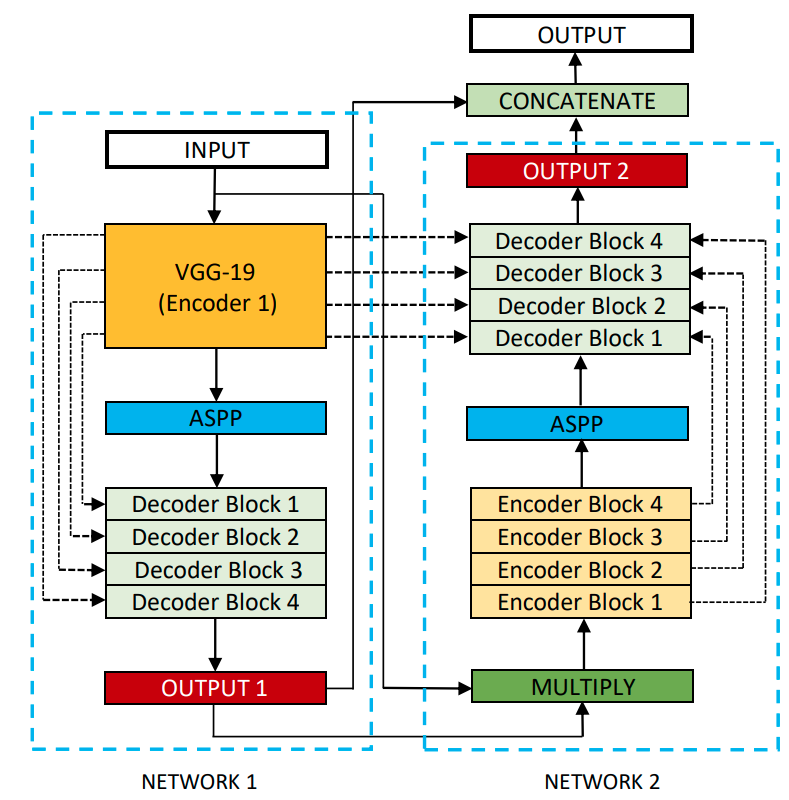
\includegraphics[width=8cm]{images/DoubleU-Net.png}
    \caption {DoubleU-Net architecture.}
    \label{fig:double_unet}
\end{figure}

What distinguishes DoubleU-Net from U-Net in the first network (NETWORK1) is the use of VGG-19 marked in yellow, ASPP marked in blue, and decoder block marked in light green. The squeeze-and-excite block is used in the encoder of NETWORK 1 and decoder blocks of NETWORK 1 and NETWORK 2. An element-wise multiplication is performed between the output of NETWORK 1 with the input of the same network. The difference between DoubleU-Net and U-Net in the second network (NETWORK 2) is only the use of ASPP and squeeze-and-excite block. All other components remain the same.

At the original paper \cite{Jha2020} it was concluded the experimental results shows that DoubleU-Net achieved a DSC of $0.7649$ and a mIoU of $0.6255$ what is better rather then U-net and the rest baseline algorithms. 

\section{Summary}
The applications of the classical techniques and traditional machine learning methods, such as region growing, edge detection based algorithms and clustering in medical image classification began long ago. 

However, each certain method has disadvantages which I had narrated above. To sum them up, the performance is far from the practical standard and the developing of them is quite slow in recent years. Likewise, the feature extracting and selection are time-consuming and vary according to different objects. The advent of deep neural networks, especially the CNNs hugely impacted in changing image classification tasks and had achieved significant performance since 2012.

Some research on medical image classification by CNN has achieved performances rivaling human experts. It was perfectly demonstrated in the recent research work \cite{Anwar2018} that indeed the CNN based methods can achieve highly precise accuracy in various tasks such as classification and segmentation. 

As it was noticed in one of  \href{https://www.itnonline.com/content/deep-learning-medical-imaging-create-300-million-market-2021}{"Image Technology News"} journal articles: ``Deep learning is a truly transformative technology and the longer-term impact on the radiology market should not be underestimated. It’s more a question of when, not if, machine learning will be routinely used in imaging diagnosis``. 


